\section{Proposed Traffic Classification Method}
\label{sec:Proposed_Traffic_Classification_Method}
\begin{figure*}[htbp]
	\centering
	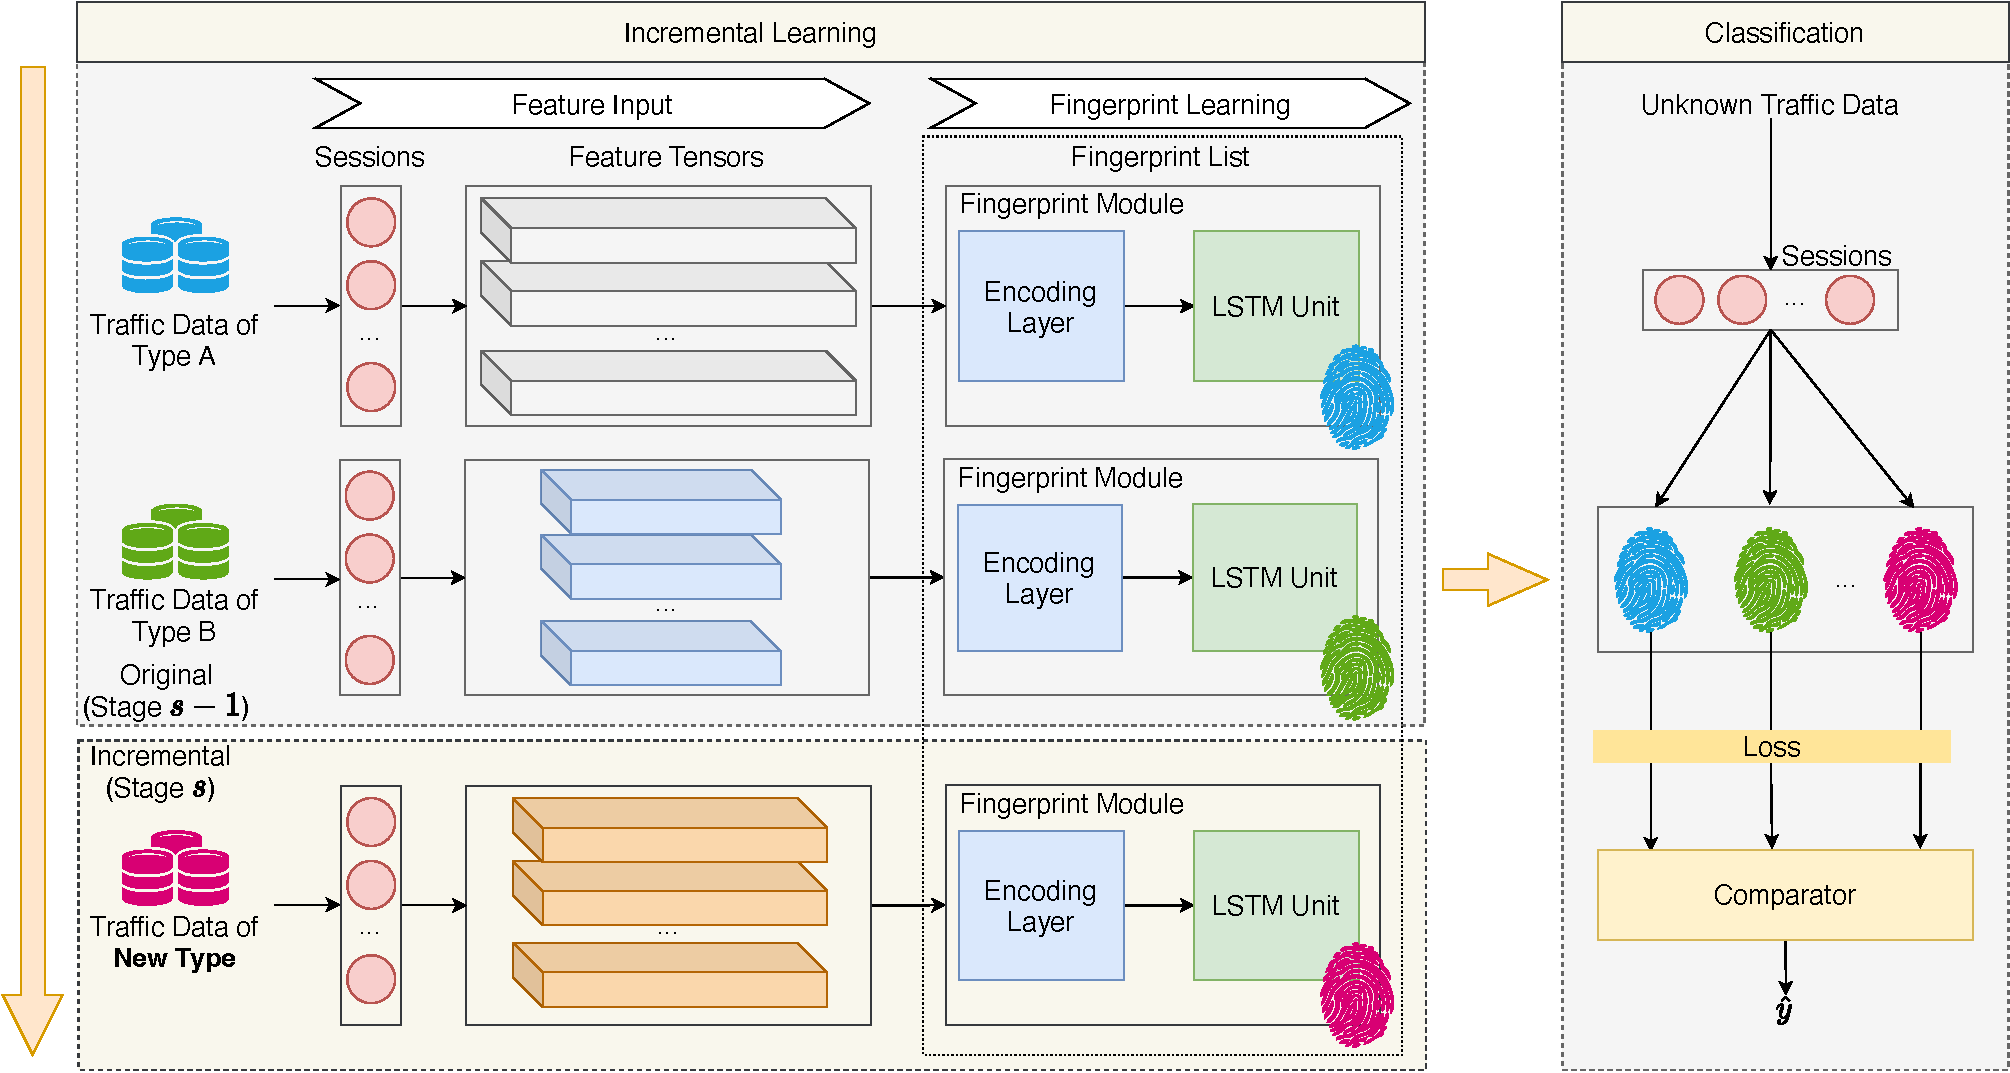
\includegraphics[scale=0.45]{figs/overview_of_model.pdf}
	\caption{Overview of \sys.}
	\label{fig:overview_of_model}
\end{figure*}

\subsection{Overview}
In Section~\ref{sec:Introduction} and Section~\ref{sec:Preliminaries}, we have discussed the limitations of current encrypted traffic classification methods, which motivate us to carry out further studies.
Here we briefly summarize the limitations and motivations as the following two points. 

\first \textit{Current methods for encrypted traffic classification are not suitable for incremental learning.} 
These methods assume the training data for all categories is available at the time of initial training. 
However, it will always emerge new attacks in real-world situations. 
This motivates us to design an incremental model.

\second \textit{Current methods for encrypted traffic classification are not interpretable.} 
The inference process of these methods is under a black-box setting and lacks interpretability. 
However, we need to understand how the model comes to specific conclusions and 
what the model learns.

Based on the above limitations and motivations, we propose the \sys. 
The two main design principles are as follows:

\first \textit{\sys learns the fingerprints of traffic and is interpretable.}
The training process of \sys does not directly implement a traditional classification task. 
Instead, each LSTM unit learns the \emph{fingerprint} (behavioral characteristics) of the input samples. 
In other words, at each time step, the current output of each LSTM unit is as close as possible to the next input of the sequence. 
This learning process is different from the typical classification task which calculates cross-entropy loss at the last time step as described in Section~\ref{sec:Preliminaries}.
We term this training process \emph{fingerprint learning}. 
By such replacement, our \sys has local robustness and is adaptive to imbalanced data.
Moreover, we can rank time-series features, identify import features in prediction and calculate the inter-class distance between different traffic types based on the learning process. 
These capabilities enhance the interpretability of \sys and will be demonstrated in Section~\ref{sec:Model_Interpretability}. 

\second \textit{\sys is an incremental model.} 
It contains multiple independent fingerprint modules. 
Each module maintains a set of parameters and corresponds to the \emph{fingerprint} of a specific traffic type. 
Therefore, we only need to train a set of additional parameters for the newly introduced traffic type. 
Such a design indicates that \sys could be deployed as an incremental model. 

The overview of \sys is depicted in Fig.~\ref{fig:overview_of_model}. 
The whole process of \sys includes incremental learning and classification. 
Further, the workflow of incremental learning can be divided into feature input and incremental fingerprint learning. 
We will discuss each part in detail below.

\subsection{Feature Input}
The first part is feature input. 
In this process, we extract feature tensors from raw traffic data.
We first split the raw traffic data of each traffic type into sessions and then perform feature extraction on each packet in sessions.

For formalization, suppose we have raw traffic data $D$ and we split it into $N$ sessions.
Each session is a sample and is composed of bi-directional packets with the same IP, port, and transport layer protocol.
The feature tensors are extracted from the first $T$ packets in each session and are composed of the packet feature vectors. 
Each packet feature vector consists of packet length, direction, the interval of arrival time, and values of fields in the packet header, \eg TTL (Time To Live), TCP flags, and TCP window size. 
Therefore, the feature tensor of the $p$-th sample can be denoted as $\mathbf{x^{(p)}} = [\mathbf{L_1^{(p)}}, \mathbf{L_2^{(p)}}, ..., \mathbf{L_T^{(p)}}]$, where $T$ is the time sequence length of each sample and $\mathbf{L_i^{(p)}} \in \mathbb{R}^d$ is the $d$-dimensional packet feature vector at time step $i$. 

Particularly, the flexibility of our feature input is that we can select different features and different time sequence lengths for each traffic type, \ie $d$ and $T$ can be different for various traffic types.  
In other words, the feature input process is not dependent on the fixed number of traffic types. 
When a new traffic type is added, we can select the appropriate features and time sequence length for this newly added traffic type without affecting those of existing traffic types.
This property of the feature input process creates the conditions for incremental fingerprint learning.

\subsection{Incremental Fingerprint Learning}
The second part is incremental fingerprint learning. 
In this process, we learn the fingerprints of different traffic types in an incremental manner.

Different from the model training process of typical classification tasks with LSTM, \sys aims to train a model which can learn \emph{fingerprints} (behavioral characteristics) of each traffic type. 
We call this process \emph{fingerprint learning}. 
As described in previous sections, we use fingerprint LSTM instead of traditional LSTM to model the packet sequence in sessions of a traffic type, which has local robustness and is suitable for an imbalanced dataset.

In addition, we add an encoding layer before fingerprint LSTM to constitute a fingerprint module.
The encoding layer takes the original feature tensors as input and generates the latent representations.
It simply uses a linear layer with the $\mathit{tanh}$ activation function.
There are two benefits of adding an encoding layer.
\first Some fields in the packet headers are categorical features, \eg TCP Flags (SYN, ACK, etc). The encoding layer can transform these features into numerical features, which are more convenient for computation.
\second There may be redundant information in the original features. 
The encoding layer can reduce the redundant information, which helps the model learn the fingerprints of network traffic better. 

Moreover, the \sys maintains a fingerprint list. 
As depicted in Fig.~\ref{fig:overview_of_model}, there are multiple fingerprint modules in the fingerprint list. 
Each fingerprint module maintains an \emph{independent} set of parameters that corresponds to a traffic type.
This means that \sys is designed in an incremental learning manner. 
In other words, the only thing that needs to be done for having the ability to recognize a new traffic type is to introduce an additional fingerprint module to the fingerprint list and to train this module with the new traffic data.
This provides \sys the capability to classify new traffic types, without retraining existing fingerprint modules.

The entire algorithm of incremental fingerprint learning is exhibited in Algorithm~\ref{alg:incremental_fingerprint_learning}.
\begin{algorithm}[H]
\caption{Incremental Fingerprint Learning.}
\label{alg:incremental_fingerprint_learning}
\renewcommand{\algorithmicrequire}{\textbf{Input:}}
\renewcommand{\algorithmicensure}{\textbf{Output:}}
\begin{algorithmic}[1]
\REQUIRE $X^s, \psi^{s-1}$
\STATE Create a new fingerprint module $[\rho^s, \Omega^s]$
\STATE Initialize the parameters of $[\rho^s$, $\Omega^s]$ randomly
\FOR{$\mathbf{x^{(p)}} \in D^s$} 
	\STATE $\mathbf{e^{(p)}} \gets \rho^s(\mathbf{x^{(p)}}) $
	\STATE $\mathbf{a^{(p)}} \gets \Omega^s(\mathbf{e^{(p)}})$
	\STATE $\mathcal{L}(\mathbf{x^{(p)}}) \gets \frac{1}{T-1} \sum_{t=1}^{T-1}\vert\vert \mathbf{a_t^{(p)}} - \mathbf{L_{t+1}^{(p)}} \vert\vert $
	\STATE Calculate the gradient of parameters of $[\rho^s, \Omega^s]$
	\STATE Update the parameters of $[\rho^s, \Omega^s]$
\ENDFOR
\STATE $\psi^s \gets $ append $[\rho^s, \Omega^s]$ to the fingerprint list of $\psi^{s-1}$
\ENSURE $\psi^{s}$
\end{algorithmic}
\end{algorithm}

In an incremental learning scenario, we introduce a new traffic type using training samples $X^s$.
After the incremental fingerprint learning, the previous stage model $\psi^{s-1}$ becomes $\psi^s$, which has the ability to classify the new traffic type.
The first step of incremental fingerprint learning is to create a new fingerprint module, which consists of an encoding layer $\rho^s$ and a fingerprint LSTM $\Omega^s$ (line 1).
Then we randomly initialize the parameters of each component of the fingerprint module (line 2). 
In each iteration, we sequentially feed the training samples into the encoding layer and the fingerprint LSTM (lines 4-5). 
The learning process aims to make the output $\mathbf{a_t^{(p)}}$ as close as possible to the next input $\mathbf{L_{t+1}^{(p)}}$ at $t$-th time step,  where $1 \le t \le T-1 $ (line 6). 
Therefore, the loss function of the $p$-th sample can be set as follow: 
\begin{equation}\label{eq:lossfunction}
    \mathcal{L}(\mathbf{x^{(p)}}) = \frac{1}{T-1} \sum_{t=1}^{T-1}\vert\vert \mathbf{a_t^{(p)}} - \mathbf{L_{t+1}^{(p)}} \vert\vert
\end{equation}
After the calculation of loss, we can obtain the gradient of the parameters of the fingerprint module with backpropagation (line 7). 
Then we update the parameters of the fingerprint module (line 8).
We can get the new model $\psi^s$ after iterations over all training samples (line 10).

\subsection{Traffic Classification}
The third part is the traffic classification. 
When the unknown traffic data arrives,  we first process the data with feature input, which converts the raw traffic data into feature tensors. 
Then we feed feature tensors to each fingerprint module in the fingerprint list that is trained in the incremental fingerprint learning part.
Each fingerprint module calculates the loss defined in Eq.~(\ref{eq:lossfunction}).
Since each fingerprint module has learned the \emph{fingerprint} of a specific traffic type, it will output a small loss for traffic with exactly the same type while giving a relatively large loss for the sample of other traffic types. 
Consequently, the unknown traffic is classified as the corresponding type of the fingerprint module with the minimum loss.
This process is represented as a \emph{comparator} in Fig.~\ref{fig:overview_of_model}.
To formulate this process, suppose that $\mathcal{L}_i(\mathbf{x^{(p)}})$ represents the output loss of $p$-th unknown traffic sample calculated by $i$-th fingerprint module in the fingerprint list. We can classify the sample as $\hat{y_p}$ by determining the specific $i$ which makes $\mathcal{L}_i(\mathbf{x^{(p)}})$ minimum,
\begin{equation}\label{eq:argminlabel}
\hat{y_p} = \mathop{\arg\min}\limits_{i}  \mathcal{L}_i(\mathbf{x^{(p)}})
\end{equation}
